\documentclass[journal,12pt,twocolumn]{IEEEtran}
\def\inputGnumericTable{}
\usepackage{setspace}
\usepackage{gensymb}
\usepackage{xcolor}
\usepackage{caption}
\singlespacing
\usepackage{siunitx}
\usepackage[cmex10]{amsmath}
\usepackage{mathtools}
\usepackage{hyperref}
\usepackage{amsthm}
\usepackage{mathrsfs}
\usepackage{txfonts}
\usepackage{stfloats}
\usepackage{cite}
\usepackage{cases}
\usepackage{subfig}
\usepackage{longtable}
\usepackage{multirow}
\usepackage{enumitem}
\usepackage{mathtools}
\usepackage{listings}
\usepackage{tikz}
\usetikzlibrary{shapes,arrows,positioning}
\usepackage{circuitikz}
       \usepackage[latin1]{inputenc}
       \usepackage{fullpage}
       \usepackage{color}
       \usepackage{array}
       \usepackage{longtable}
       \usepackage{calc}
       \usepackage{multirow}
       \usepackage{hhline}
       \usepackage{ifthen}
	   \usepackage{setspace}
\let\vec\mathbf
\DeclareMathOperator*{\Res}{Res}
\renewcommand\thesection{\arabic{section}}
\renewcommand\thesubsection{\thesection.\arabic{subsection}}
\renewcommand\thesubsubsection{\thesubsection.\arabic{subsubsection}}

\renewcommand\thesectiondis{\arabic{section}}
\renewcommand\thesubsectiondis{\thesectiondis.\arabic{subsection}}
\renewcommand\thesubsubsectiondis{\thesubsectiondis.\arabic{subsubsection}}
\hyphenation{op-tical net-works semi-conduc-tor}

\lstset{
language=Python,
frame=single, 
breaklines=true,
columns=fullflexible
}
\begin{document}
\theoremstyle{definition}
\newtheorem{theorem}{Theorem}[section]
\newtheorem{problem}{Problem}
\newtheorem{proposition}{Proposition}[section]
\newtheorem{lemma}{Lemma}[section]
\newtheorem{corollary}[theorem]{Corollary}
\newtheorem{example}{Example}[section]
\newtheorem{definition}{Definition}[section]
\newcommand{\BEQA}{\begin{eqnarray}}
        \newcommand{\EEQA}{\end{eqnarray}}
\newcommand{\define}{\stackrel{\triangle}{=}}
\newcommand{\myvec}[1]{\ensuremath{\begin{pmatrix}#1\end{pmatrix}}}
\newcommand{\mydet}[1]{\ensuremath{\begin{vmatrix}#1\end{vmatrix}}}

\bibliographystyle{IEEEtran}
\providecommand{\nCr}[2]{\,^{#1}C_{#2}} % nCr
\providecommand{\nPr}[2]{\,^{#1}P_{#2}} % nPr
\providecommand{\mbf}{\mathbf}
\providecommand{\pr}[1]{\ensuremath{\Pr\left(#1\right)}}
\providecommand{\qfunc}[1]{\ensuremath{Q\left(#1\right)}}
\providecommand{\sbrak}[1]{\ensuremath{{}\left[#1\right]}}
\providecommand{\lsbrak}[1]{\ensuremath{{}\left[#1\right.}}
\providecommand{\rsbrak}[1]{\ensuremath{{}\left.#1\right]}}
\providecommand{\brak}[1]{\ensuremath{\left(#1\right)}}
\providecommand{\lbrak}[1]{\ensuremath{\left(#1\right.}}
\providecommand{\rbrak}[1]{\ensuremath{\left.#1\right)}}
\providecommand{\cbrak}[1]{\ensuremath{\left\{#1\right\}}}
\providecommand{\lcbrak}[1]{\ensuremath{\left\{#1\right.}}
\providecommand{\rcbrak}[1]{\ensuremath{\left.#1\right\}}}
\theoremstyle{remark}
\newtheorem{rem}{Remark}
\newcommand{\sgn}{\mathop{\mathrm{sgn}}}
\newcommand{\rect}{\mathop{\mathrm{rect}}}
\newcommand{\sinc}{\mathop{\mathrm{sinc}}}
\providecommand{\abs}[1]{\left\vert#1\right\vert}
\providecommand{\res}[1]{\Res\displaylimits_{#1}}
\providecommand{\norm}[1]{\lVert#1\rVert}
\providecommand{\mtx}[1]{\mathbf{#1}}
\providecommand{\mean}[1]{E\left[ #1 \right]}
\providecommand{\fourier}{\overset{\mathcal{F}}{ \rightleftharpoons}}
\providecommand{\ztrans}{\overset{\mathcal{Z}}{ \rightleftharpoons}}
\providecommand{\system}[1]{\overset{\mathcal{#1}}{ \longleftrightarrow}}
\newcommand{\solution}{\noindent \textbf{Solution: }}
\providecommand{\dec}[2]{\ensuremath{\overset{#1}{\underset{#2}{\gtrless}}}}
\let\StandardTheFigure\thefigure
\def\putbox#1#2#3{\makebox[0in][l]{\makebox[#1][l]{}\raisebox{\baselineskip}[0in][0in]{\raisebox{#2}[0in][0in]{#3}}}}
\def\rightbox#1{\makebox[0in][r]{#1}}
\def\centbox#1{\makebox[0in]{#1}}
\def\topbox#1{\raisebox{-\baselineskip}[0in][0in]{#1}}
\def\midbox#1{\raisebox{-0.5\baselineskip}[0in][0in]{#1}}

\vspace{3cm}
\title{\LaTeX\ 9.10.5.3}
\author{Lokesh Surana}
\maketitle
\section*{Class 9, Chapter 10, Exercse 5.3}

Q. $\angle{PQR} = 100\degree$, where $\vec{P}, \vec{Q}$ and $\vec{R}$ are points on a circle with centre $\vec{O}$. Find $\angle{OPR}$

\solution
Let, we have a unit circle with center at origin, i.e. $\vec{O}$, and radius $r = 1$.
Then let following points be on the circle

\begin{table}[ht!]
    \begin{tabular}{|c|c|p{5cm}|}
\hline
\textbf{Symbol} & \textbf{Value} & \textbf{Description} \\
\hline
$\theta$ & $30\degree$ & $\angle{BAP} = \angle{BAQ}$ \\
\hline
$a$ & $9$ & $AB$ \\
\hline
$c$ & $8$ & $AQ$ \\
\hline
$\vec{e}_1$ & $\myvec{1\\0}$ & Basis vector \\
\hline
\end{tabular}

    \caption{points}
    \label{tab:points}
\end{table}

Using the theorem from appendix of matrix analysis book,
Let 
\begin{align}
\vec{P} =  \myvec{\cos \theta_1 \\ \sin \theta_1},
\vec{Q} =  \myvec{\cos \theta_2 \\ \sin \theta_2},
\vec{R} =  \myvec{\cos \theta \\ \sin \theta},
\end{align}
 be points on  a unit circle. Then
\begin{align}
  \cos\angle{PRQ} &= \frac{\brak{\vec{R}-\vec{P}}^{\top} \brak{\vec{R}-\vec{Q}}}{\norm{\vec{R}-\vec{P}}\norm{\vec{R}-\vec{Q}}}
  \\
  &= \cos \brak{\frac{\theta_1 - \theta_2}{2}}
\end{align}


For our question we have 3 points
\begin{align}
    \vec{P} =  \myvec{\cos \theta   \\ \sin \theta},
    \vec{Q} =  \myvec{\cos \brak{-\frac{\pi}{6}} \\ \sin \brak{-\frac{\pi}{6}}},
    \vec{R} =  \myvec{\cos 0 \\ \sin 0},
\end{align}
on a unit circle. Then using this theorem, we get

\begin{align}
    \label{eq:1} \cos\angle{PQR} & = \frac{\brak{\vec{Q}-\vec{P}}^{\top} \brak{\vec{Q}-\vec{R}}}{\norm{\vec{Q}-\vec{P}}\norm{\vec{Q}-\vec{R}}}\\
    & = \cos \brak{\frac{\theta - 0}{2}}
\end{align}

As per given condition, we have
\begin{align}
    \angle{PQR}                          & = 100\degree                                                                                                      \\
    \implies \cos100\degree & =  \cos \brak{\frac{\theta - 0}{2}}\\
    \theta  & =   200\degree                \\
    \vec{P} & = \myvec{\cos200\degree \\ \sin200\degree}
\end{align}

\begin{figure}[!htb]
    \centering
    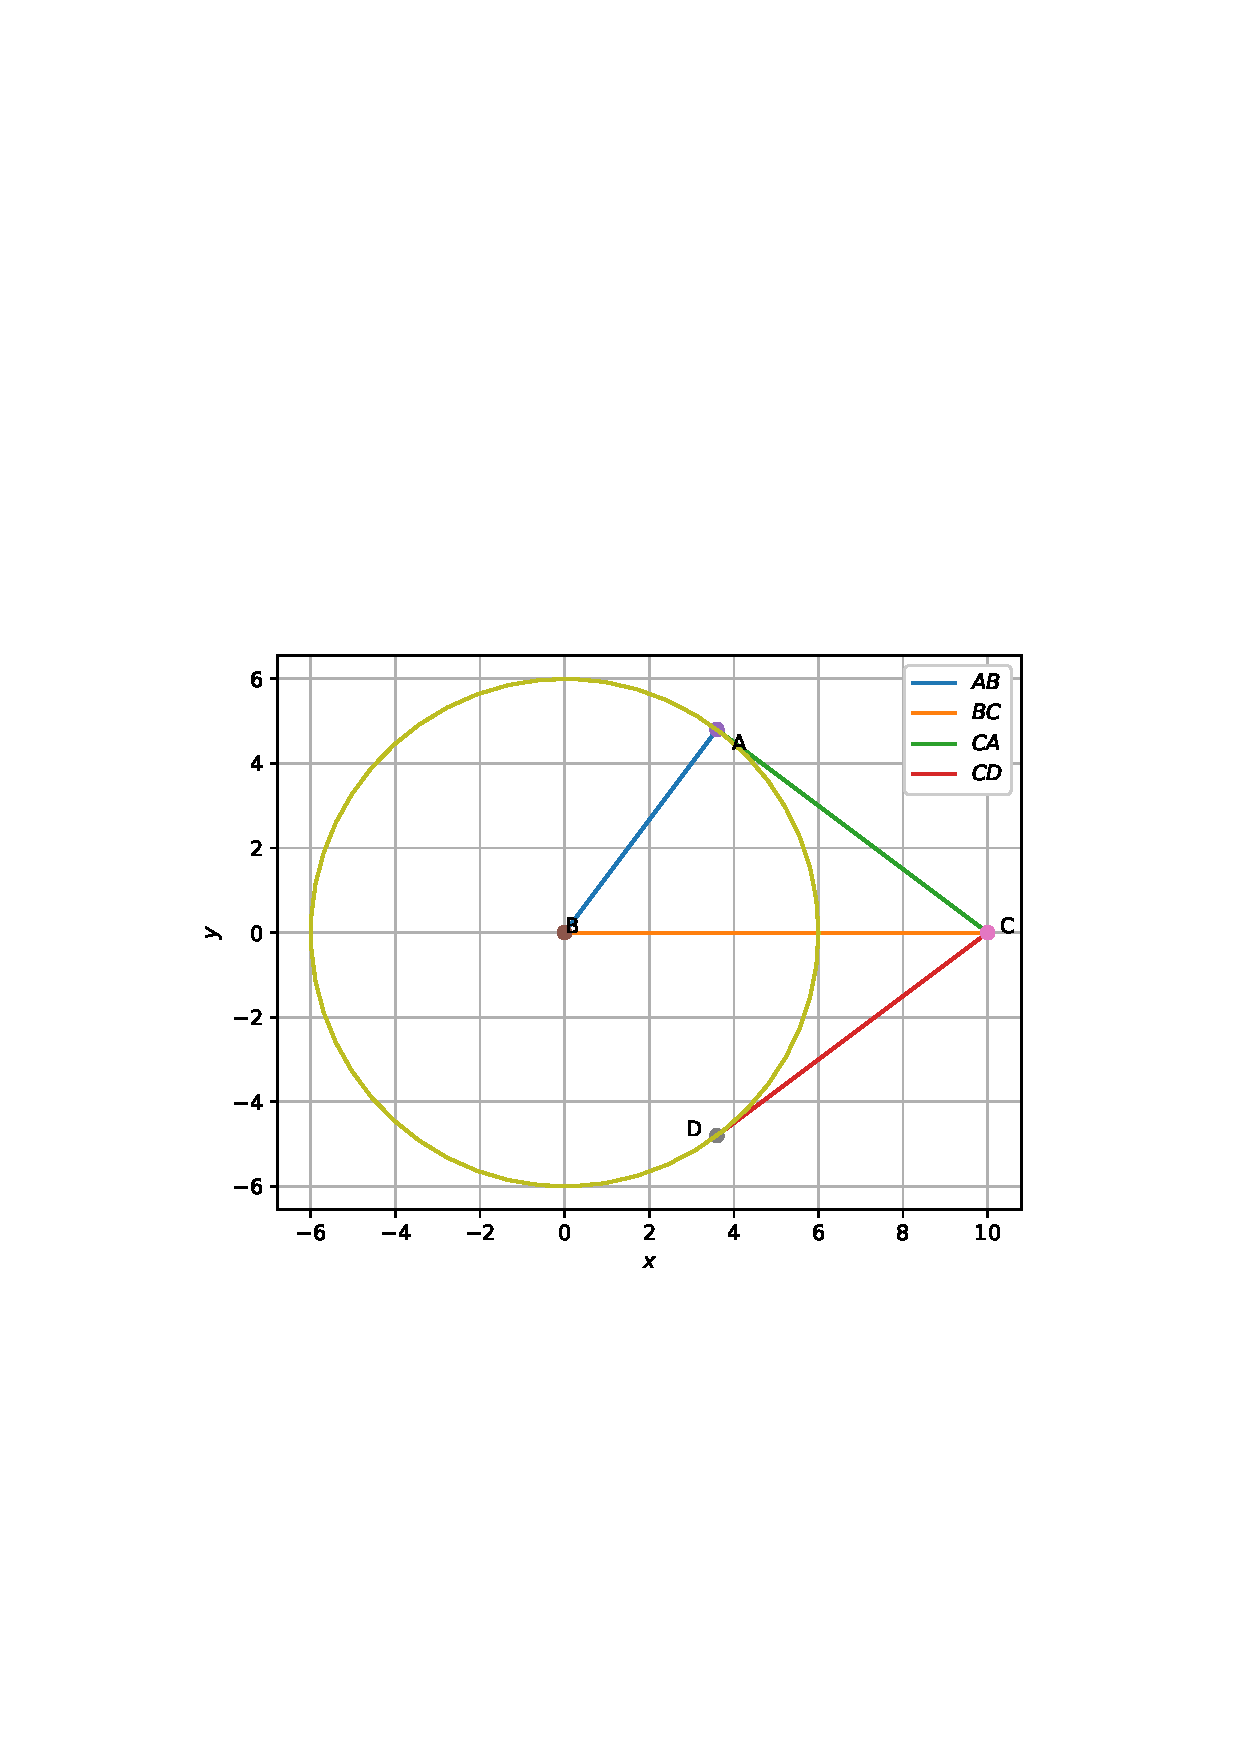
\includegraphics[width=\columnwidth]{figs/circle.png}
    \caption{circle}
    \label{fig:circle}
\end{figure}

Now, let's check the $\angle{OPR}$
\begin{align}
    \cos\angle{OPR} = \frac{\brak{\vec{P}-\vec{O}}^{\top} \brak{\vec{P}-\vec{R}}}{\norm{\vec{P}-\vec{O}}\norm{\vec{P}-\vec{R}}}\\
\end{align}

\begin{align}
    \norm{\vec{P}-\vec{O}} &= \sqrt{\brak{\cos^2 200\degree + \sin^2 200\degree}} = 1\\
    \norm{\vec{P}-\vec{R}} &= \sqrt{\brak{\cos200\degree - 1}^2 + \brak{\sin^2 200\degree}}\\
    &= 2\sin100\degree
\end{align}

So,
\begin{align}
    \cos\angle{OPR} &= \frac{\myvec{\cos200\degree\\\sin200\degree}\myvec{\cos200\degree - 1&\sin200\degree}}{2\sin100\degree}\\
    &= \frac{1 - \cos200\degree}{2\sin100\degree}\\
    &= \sin100\degree
\end{align}

\begin{align}
    \implies \angle{OPR} &= \cos^{-1} \sin100\degree = 10\degree
\end{align}
\end{document}